%%%%%%%%%%%%%%%%%%%%%%%%%%%%%%%%%%%%%%%%%%%%%%%%%%%%%%%%%%%%%%%%%%%%%%%%%%%%%%%%
%2345678901234567890123456789012345678901234567890123456789012345678901234567890
%        1         2         3         4         5         6         7         8

\documentclass[letterpaper, 10 pt, conference]{ieeeconf}  % Comment this line out if you need a4paper

%\documentclass[a4paper, 10pt, conference]{ieeeconf}      % Use this line for a4 paper

\IEEEoverridecommandlockouts                              % This command is only needed if 
                                                          % you want to use the \thanks command

\overrideIEEEmargins                                      % Needed to meet printer requirements.

% See the \addtolength command later in the file to balance the column lengths
% on the last page of the document

% The following packages can be found on http:\\www.ctan.org
\usepackage{graphics} % for pdf, bitmapped graphics files
\usepackage{epsfig} % for postscript graphics files
%\usepackage{mathptmx} % assumes new font selection scheme installed
%\usepackage{times} % assumes new font selection scheme installed
%\usepackage{amsmath} % assumes amsmath package installed
%\usepackage{amssymb}  % assumes amsmath package installed
\usepackage{booktabs}
\usepackage{graphicx}
\usepackage{siunitx}

\title{\LARGE \bf
Soft Wearable Augmented Walking Suit with Pneumatic Gel Muscles and Stance Phase Detection System to Assist Gait
}



\author{Chetan Thakur$^{1}$ Kazunori Ogawa$^{1,2}$ Toshio Tsuji$^{1}$ Yuichi Kurita$^{1}$% <-this % stops a space
\thanks{*The author (Chetan Thakur) was supported through the Hiroshima University
TAOYAKA Program for creating a flexible, enduring, peaceful society, funded by the Program for Leading
Graduate Schools, Ministry of Education, Culture, Sports, Science and Technology.}% <-this % stops a space
\thanks{$^{1}$Department of Systems Cybernetics, Graduate School of Engineering,
	Hiroshima University, Hiroshima, Japan
        {\tt\small }}%
\thanks{$^{2}$Daiya Industries Co. Ltd. Japan
        {\tt\small }}%
}


\begin{document}
\special{papersize=8.5in,11in}
\setlength{\pdfpageheight}{11in}
\setlength{\pdfpagewidth}{8.5in}

\maketitle
\thispagestyle{empty}
\pagestyle{empty}

\maketitle
\thispagestyle{empty}
\pagestyle{empty}


%%%%%%%%%%%%%%%%%%%%%%%%%%%%%%%%%%%%%%%%%%%%%%%%%%%%%%%%%%%%%%%%%%%%%%%%%%%%%%%%
\begin{abstract}

Lower limb of the human body is responsible for human locomotion and maintain a good quality of life. However, there are many instances of muscle fatigue or injuries happens due to the stressful work environment, aging and work that involve walking a long distance. Therefore, there is a need for walking assistive suit which can unload muscle activation during walking and reduce the chances of lower limb muscle fatigue. In this paper we discuss the development of lightweight and wearable Augmented Walking Suit (AWS) using Pneumatic Gel Muscle (PGM) and its actuation control using lower limb pose detection mechanism by considering human gait cycle. The objective of this assistive suit is to reduce the required muscle effort of posterior and anterior muscles of lower limb during the swing phase of the gait cycle thereby making it easier to move forward. Evaluation experiment was conducted with seven subjects to record surface EMG (sEMG) of eight lower limb muscles for two levels of assistive force when wearing AWS and without wearing AWS. The statistical analysis and sEMG signal envelope of average percentage maximum voluntary contraction (\%MVC) of eight muscles for all subjects shows a significant reduction or no change in muscles activity while comparing assisted and unassisted gait.
\end{abstract}


%%%%%%%%%%%%%%%%%%%%%%%%%%%%%%%%%%%%%%%%%%%%%%%%%%%%%%%%%%%%%%%%%%%%%%%%%%%%%%%%
\section{INTRODUCTION}\label{intro}

Ability to move uninterrupted is one of the critical function of human body. It is one of the reasons for enjoying a good quality of life by enabling one to be independent for performing a variety of daily tasks. However, there are many instances such as aging, accidents and longer and more stressful working conditions that result in muscle fatigue and injuries making it difficult to walk by affecting the quality of life of the individual. Such situation can be avoided or addressed using exoskeletons or wearable assistive devices. Muscle activation pattern of human gait is dynamic, and changes as the motion or intent are changed, but the basic pattern of gait cycle is same for all. While developing Augmented Walking Suit (AWS) we considered factors such as nature of work area, age, flexibility to use in outside environment, lightweight, portable, easy to use, reduces muscle efforts during walking and no impact on regular gait cycle. With increasing elderly population, stressful work condition devices like these will play a significant role in improving the quality of life. L. Garçon et al. \cite{1} in his review mentioned there are large requirement assistive devices for mobility for people such as elderly, disabled and healthcare staff for various tasks involved in daily life. Among various lower limb assistive devices, there exists tradeoff between autonomous actuation, wearable, lightweight and affordability. HAL \cite{2} which enable walking easier for elderly and rehabilitation post stroke or accidents. Wearable agri robot \cite{3} designed for supporting farming activities and reduce muscle fatigue, it supports body posture and reduces the muscle fatigue. Walking assist device with body weight support system \cite{4} for augmenting walking and assistive squats motion required for pick and place tasks in the various work environment. RoboKnee \cite{5} is one DOF exoskeleton designed to support human locomotion such as walk and stair climbing. Plantarflexion assist exoskeleton \cite{6} is designed to reduce the metabolic cost of walking.

A tethered bilateral hip extension and plantarflexion exosuit \cite{7} evaluated assistance magnitude and changes in the metabolic cost of walking and found a reduction in metabolic energy by 22.8\% while walking. Soft exosuit for hip assistance which provides 30\% of biological torque moment for gait \cite{8} by using spooled-webbing actuator connected to the back of the thigh. The Myosuit, an untethered biarticular exosuit reduces EMG activities during sit to stand transfer +motion by 26\% \cite{9}. Unilateral exosuit support ankle plantarflexion and dorsiflexion were reported to reduce metabolic rate of gait by 16\% \cite{10}. A soft inflatable exosuit for knee rehabilitation \cite{11} reduces muscle activity in rectus femoris by 7\%. A biologically inspired soft exosuit for walking assistance \cite{12} showed an average metabolic reduction of 5.1\% during walking. The passive unpowered exoskeleton reduces metabolic cost of gait by 7\% \cite{13}.

These devices classified into segments such as healthcare, disability support and augmenting locomotion. They augment human walking significantly based on a reduction in EMG activities and metabolic rate during walking, but its use in outside environment is limited especially in agriculture and factory settings. For augmented walking wearable, lightweight, portable, easy to use and reduce muscle fatigue, these criteria are essential and together missing in assistive devices discussed above. To solve this problem previously, we developed a lightweight, low powered pneumatic gel muscle (PGM) \cite{14} as shown in Fig. \ref{fig:pgm}. PGM can generate force with 60 kPa air pressure which is not possible in McKibben pneumatic artificial muscle (PAM) \cite{15}. It is also structured in a way to be stitched to fabric or fix using velcro tapes; this makes it easy to design the assistive suit. Fig. \ref{fig:pgmelongationratio} shows the relation of supplied air pressure, generated force and maximum elongated length.

In \cite{16} we devised the concept of Unplugged Powered Suit (UPS) for walking assist using the advantage of PGM and gait cycle. UPS is a passive walking assist suit where a pump at the heel of the shoe generates air pressure required to actuate PGM during the swing phase of the gait cycle. This configuration enables limb in stance phase to generate assistive air pressure required for contralateral limb in the swing phase. The pump in the shoe can generate air pressure up to 50 kPa. The challenge of the UPS as discussed in \cite{16} are actuation delay due to the long distance between pump and PGM; unable to support walking pitch of faster than two steps per second. Another limitation of the UPS is the use of the pump in the shoe, for support multiple muscle groups and more air pressure we need more pumps in the shoe which is not suitable for use in outside environment due to possible leaks in the pump and difficult to walk with pumps in the shoe. In the \cite{16} evaluation of the UPS was done based on only four muscle of lower limb and only rectus femoris showed a reduction in muscle activity by 20\% others showed no change. To overcome these challenges of UPS we developed AWS where air tank replaces the pumps and actuation control is designed using force sensitive resistors (FSR) sensors in the shoe. This change solves the problem of supporting variable walking speed, and ability to support multiple muscle groups using additional PGM’s.

In this paper, we discuss the design and control of AWS, which improves on Unplugged Powered Suit (UPS) by keeping human gait in the loop by using gait cycle identification system for generating assistive force. In section \ref{methodology} PGM and its force characteristics, biomechanics and human gait detection system and design and configuration of the Augmented walking suit is discussed. In section \ref{Evaluation}, we discuss the evaluation criteria, experiment method setups, results of the lower limb surface EMG (sEMG) evaluation for two levels of assistive force with the comparison of average gait sEMG envelope for all subjects and statistical analysis. Section \ref{discuss} presents the discussion, conclusion and future works.



\section{Methodology} \label{methodology}

\subsection{Pneumatic Gel Muscle} \label{pgm}
\begin{figure}
	\centering
	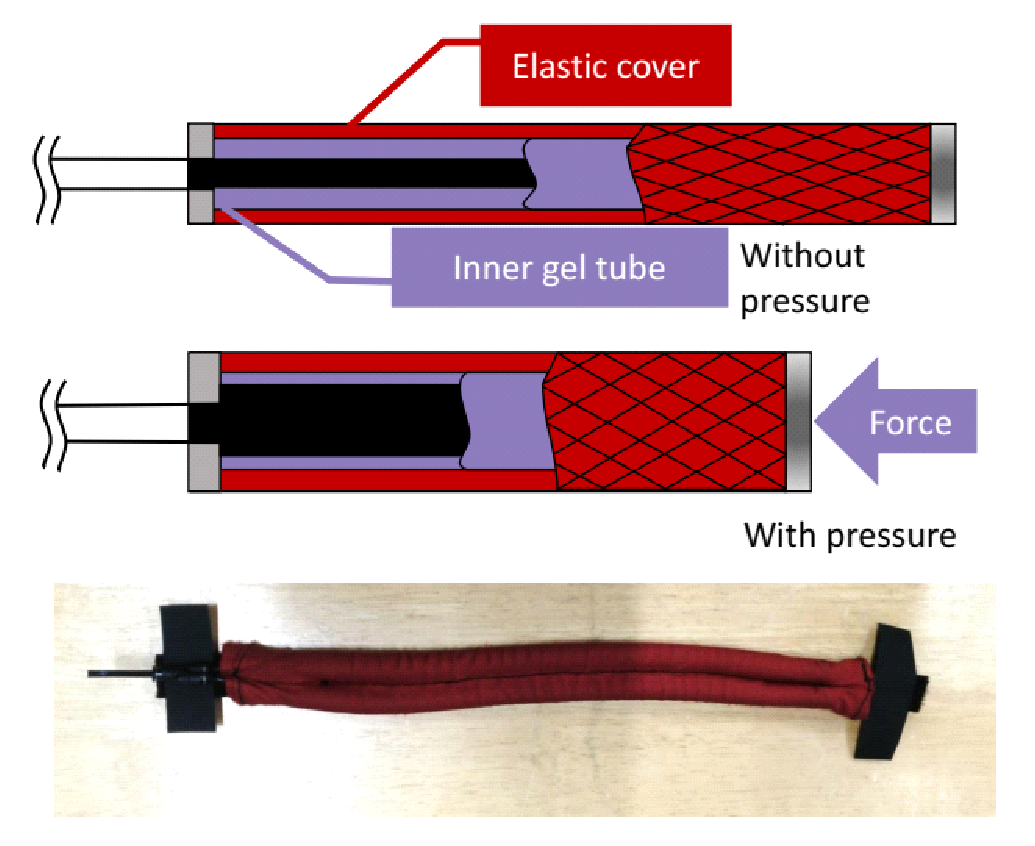
\includegraphics[width=0.9\linewidth]{../photos/pgm}
	\caption{Pneumatic Gel Muscle schematic and prototype. The inner gel tube can inflated with low air pressure to generate required force. The resting length of the prototype is 30 cm.}
	\label{fig:pgm}
\end{figure}
\begin{figure}
	\centering
	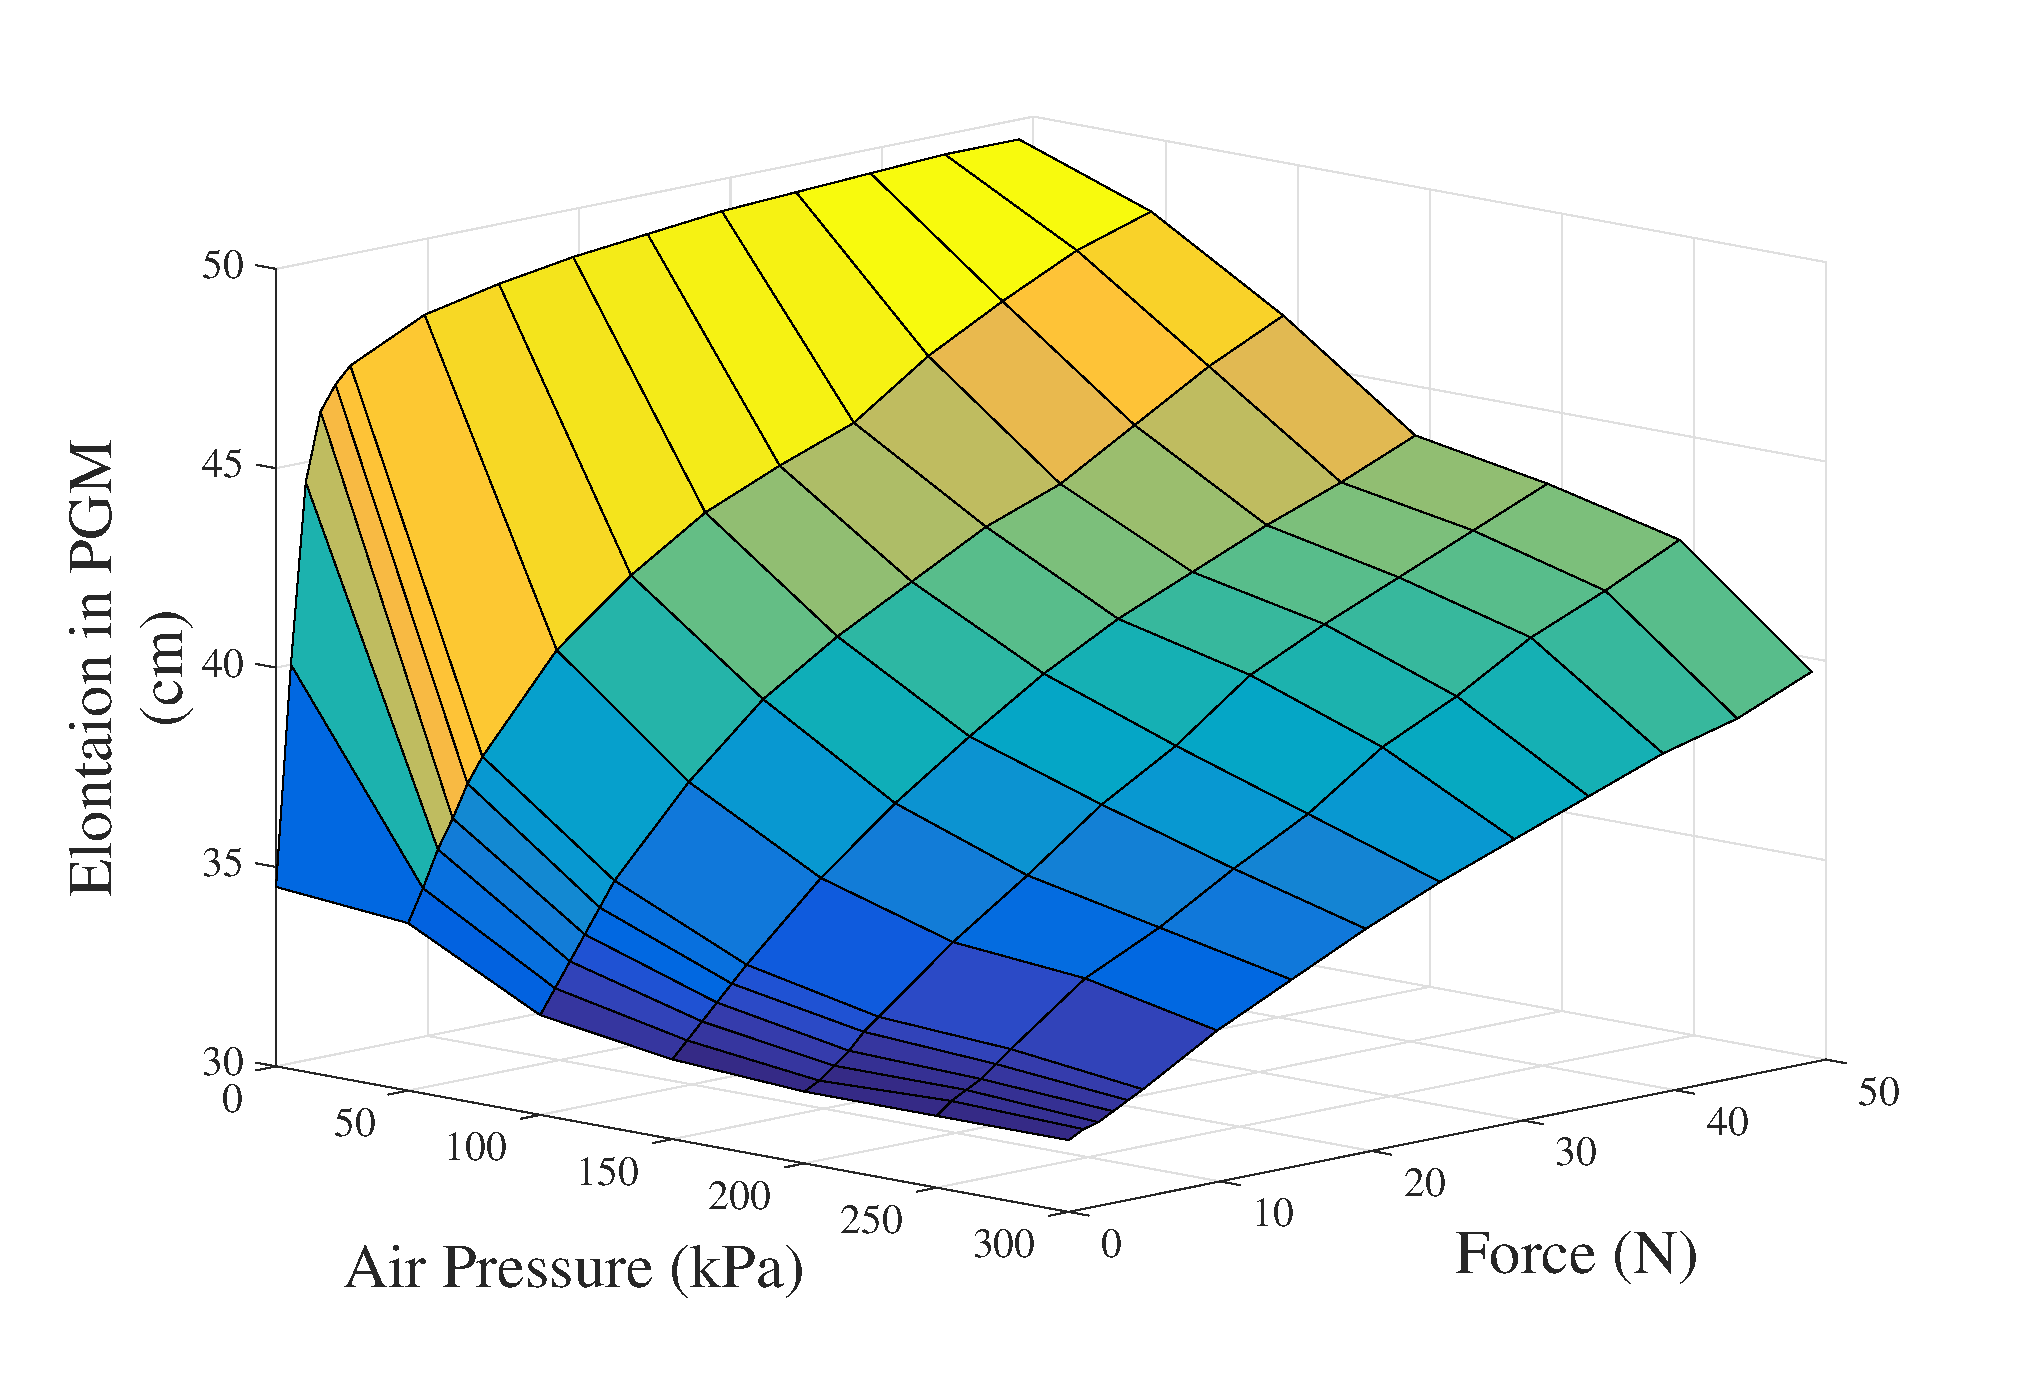
\includegraphics[width=1\linewidth]{../photos/pgmelongation}
	\caption{The graph shows relationship of elongated length of PGM, air pressure and generated force as measured in \cite{14}.}
	\label{fig:pgmelongationratio}
\end{figure}

PGM is a particular type of PAM designed to be driven by low air pressure. Fig. \ref{fig:pgm} shows schematics and real prototype of the PGM. It has a resting length of 30 cm, maximum contraction length of 25 cm and maximum elongation length of 45 cm. Construction of PGM includes an inner tube made of a unique styrene-based thermoplastic elastomer to improve the flexibility, and an outer protective mesh. McKibben PAM has rubber or silicon-based rubber tubes covered with protective mesh; these tubes need more air pressure to inflate whereas in case of PGM can generate force with air pressure as low as 50 kPa up to 300 kPa as reported by \cite{14}. The flexible design and working with low air pressure makes it more suitable choice for development of wearable assistive suits as compared to McKibben PAM who have higher force generating capacity but requires larger air pressure. Fig. \ref{fig:pgmelongationratio} shows elongation ratio of the PGM as measured by \cite{14} it shows the force-generating capacity of the PGM and elongation length for various level of air pressure. In the experiment, the one end of PGM is fixed, and test load is added to another end. Whereas in AWS both ends of the PGM is fixed and stretched, in this case, PGM’s force generating characteristics varies. This change is not measured in \cite{14}. Therefore we conducted an experiment to measure the force generated by PGM for stretched and un-stretched condition and different air pressure. The supported range of air pressure is 50 kPa to 300 kPa. Fig. \ref{fig:pgmtest} show experiment setup, where one end is connected to load cell, and at the other end air source is connected through Panasonic ADP5161 air pressure sensor. The experiment is conducted for two cases unstretched and stretched to 45 cm. Fig. \ref{fig:pgmforceprofile} shows the measured force profile for two conditions in both cases PGM shows linear force generation characteristics which are modeled as a linear equation as described in equation \ref{pgmunstreched} and \ref{pgmstreched} with their respective $R^2$ values. These models exhibit similar force generating behavior when used in AWS configuration. These characteristics are useful for controlling assistive force generated by PGM when used in AWS.

\begin{figure}
	\centering
	\includegraphics[width=1\linewidth]{../photos/forceexpsetup}
	\caption{Experiment setup for studying PGM's force profile.}
	\label{fig:pgmtest}
\end{figure}

\begin{figure}
	\centering
	\includegraphics[width=1\linewidth]{../photos/pgmforceprofile}
	\caption{PGM force profile for unstretched and stretched condition. This represents assistive force applied by PGM when used in AWS based on the input air pressure. In AWS the PGM is stretched along the length of the body segment it is attached. In our experiment we used 60 kPa and 100 kPa assistive air pressure for which approximately 30N and 44N of assistive force was applied by PGM based on the graph above.}
	\label{fig:pgmforceprofile}
\end{figure}


\begin{equation}\label{pgmunstreched}
y=0.1799x - 5.1983; (R^2=0.993)
\end{equation}
\begin{equation}\label{pgmstreched}
y = 0.3883x + 5.8899; (R^2=0.998)
\end{equation}

\subsection{Biomechanics of Gait Cycle } \label{method:gaitcycle}
AWS is designed based on human walking, i.e. gait cycle and how we walk. The gait cycle consists of three major phases, stance phase, double limb support phase and swing phase. The stance phase is responsible for weight acceptance, and load transfer to support swing phase of the contralateral limb, Fig. \ref{fig:standardgait} shows classification of the gait cycle in the stance and swing phase based on the orientation of the foot. During the transition from one phase to another, there always exists a period where both the limbs are on the ground this phase is called double limb support (DLS). In the stance phase muscle activation is observed for tibialis anterior (TA), rectus femoris (RF), vastus medialis (VM), vastus lateralis (VL), soleus (SOL), medial gastrocnemius (MG) and lateral gastrocnemius (LG). These muscles are active from heel strike until toe off in the stance phase. In the DLS phase, the limb transitioning in stance phase support the forward locomotion of the contralateral limb going in swing phase. In this phase both the limbs are on the ground for about 10\% of the one gait cycle. SOL, LG, MG and RF muscles are active and responsible for the limb going in swing phase. In the swing phase limb makes forward movement and RF, VL, VM, biceps femoris (BF) are major muscle contributors. 

During gait cycle apart from the multiple muscle activation, position and orientation of foot also change. The orientation of foot in stance phase starts from the heel strike then flat foot, heels off and ends with toe-off. Whereas in swing phase, foot orientation starts from toe-off to heel strike. In DLS foot orientation of both limb contrasts each other, i.e. one limb does heel strike, and another does toe-off. This contrast information in DLS is beneficial to identify the limbs in swing and stance phase. In following subsection \ref{method:awscontrol} we discuss how we used this information for developing assistive control of the AWS to assist swing phase of the gait cycle.


\begin{figure}
	\centering
	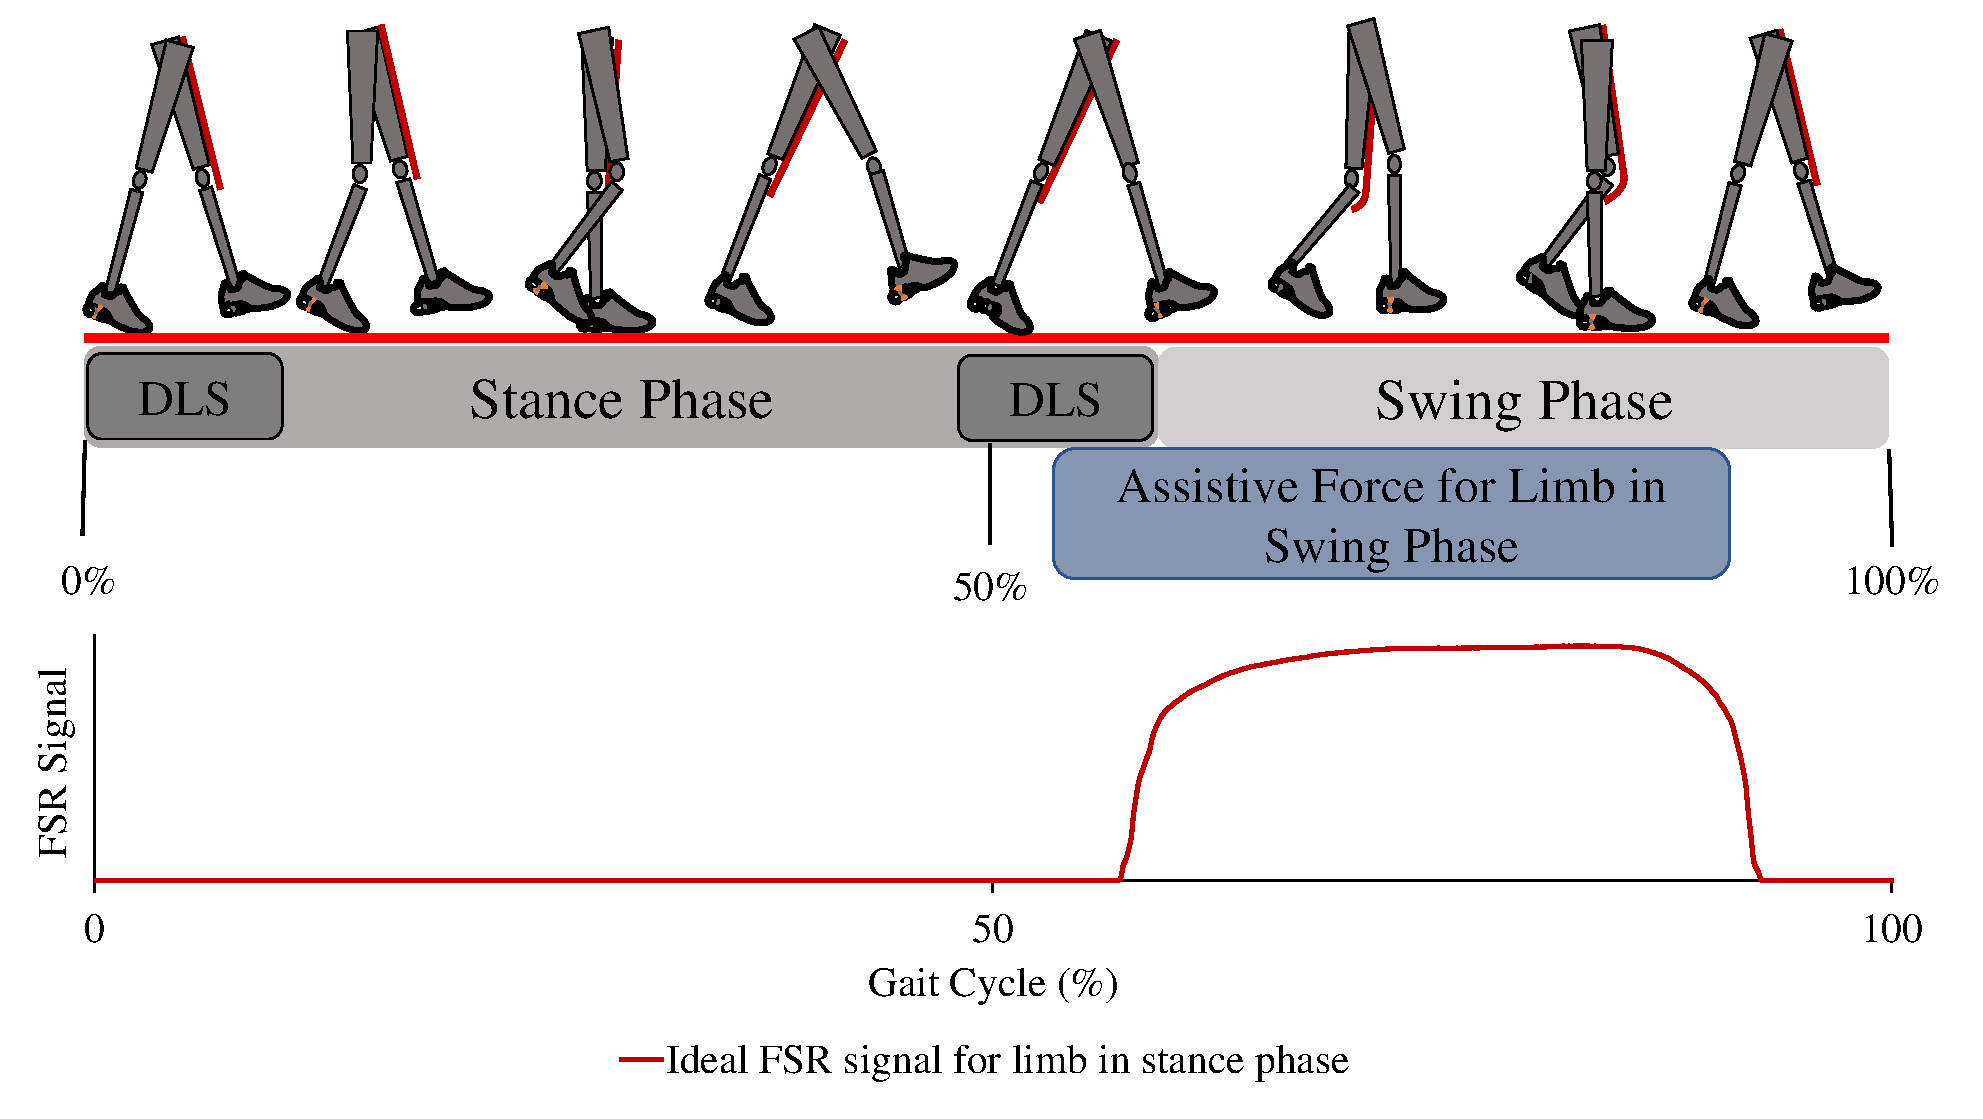
\includegraphics[width=1\linewidth]{../photos/standardGait}
	\caption{The figure shows classification of gait cycle in stance and swing phase along with the double limb support (DLS) which occurs during transition from one phase to another. It also shows the region of assistive gait which starts during double limb support just before initial swing until terminal swing phase.}
	\label{fig:standardgait}
\end{figure}

\subsection{AWS Design and Actuation Control Mechanism} \label{method:awscontrol}

AWS is designed to detect gait cycle and provide assistive force for limb in the swing phase. In the previous subsection \ref{method:gaitcycle} we talked about foot orientation in stance phase and the respective motion in the contralateral limb. We also discussed DLS and sensing the information contained in this phase is useful for controlling assistive forces generated by PGM. To sense this information, we placed force sensitive resistor (FSR) FSR-406 in the shoe to detect contrast foot orientation of both limbs in the DLS. The placement of FSR sensors is shown in Fig. \ref{fig:fsrsole}. This placement helps us identify the change in foot orientation while transitioning from stance to swing phase and vice versa in DLS phase. By utilizing the knowledge of the gait cycle and the foot orientation from FSR, we designed the assistive control mechanism for AWS. Fig. \ref{fig:awssystem} shows control mechanism of the AWS with FSR-406 sensor based stance and swing phase detection mechanism and assistive control. It is a continuous process of proportional (P) control where Arduino Uno board monitors the FSR sensor data to identify the limbs in the stance and swing phase in the gait cycle. Detection of the limb in the swing phase triggers assistive control mechanism of the PGM. For actuation control, we used Kaganei G010E1 3/2 normally closed solenoid valve. FSR sensor data is continuously monitored for switching ON/OFF solenoid valves. This system is realized using following equation

\begin{figure}
	\centering
	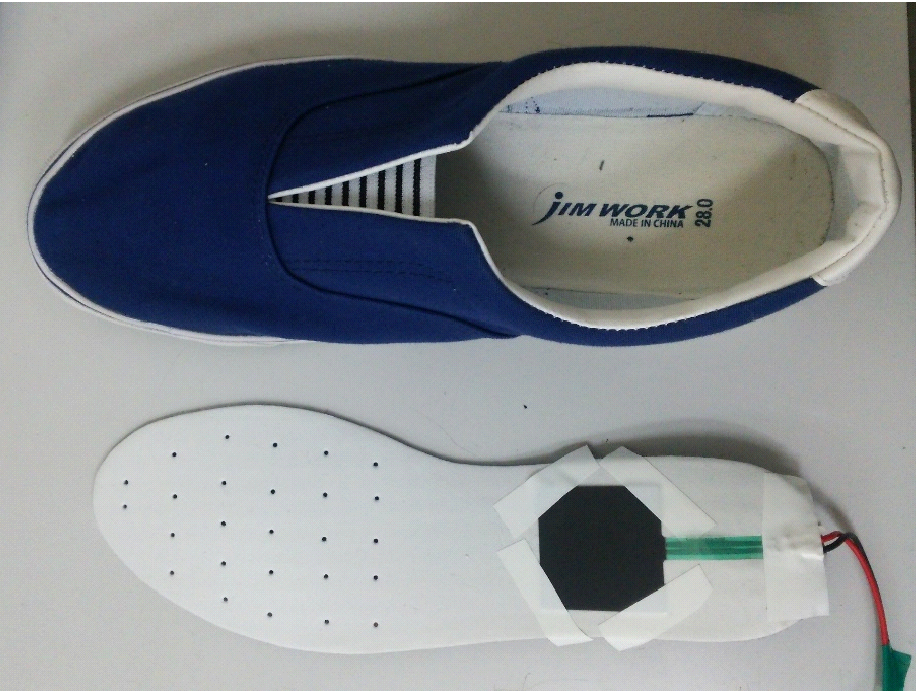
\includegraphics[width=0.3\linewidth]{../photos/fsrsole}
	\caption{The figure shows FSR-406 pressure sensor placement in the shoe. This placement detects the limb in stance and swing phase during DLS}
	\label{fig:fsrsole}
\end{figure}

\begin{figure}
	\centering
	\includegraphics[width=1\linewidth]{../photos/awscontrol}
	\caption{The figure shows AWS assist control mechanism as a continuous process of Proportional (P) control which uses FSR sensor in the shoe to actuate PGM switching on pneumatic valves connected to portable air tank.}
	\label{fig:awssystem}
\end{figure}
\begin{equation}\label{kevalue}
E = R - Y 
\end{equation}
\begin{equation}\label{uvalue}
U = kpE
\end{equation}

where $E$ is error signal, $R$ is calibrated threshold value of the FSR sensor, and $Y$ is the analog value of the FSR sensor, $U$ is input to the solenoid valve and $kp$ is the P-gain. 

The assistive control mechanism detects gait cycle by sensing the transition from one phase to another on both limbs in DLS. This way we avoid unwanted assistive forces when the user is not walking. The assistive force generated by the AWS is directly proportional to the supplied air pressure. The supplied air pressure is controlled using the regulator attached to small air tank used as a source of air pressure.  

\begin{figure}
	\centering
	\includegraphics[width=1\linewidth]{../photos/awsbigfont}
	\caption{The figure shows a subject wearing proposed AWS. The suit consists of backpack with controller, battery and air tank, waist support belt, knee support, two PGMs, pneumaitic valves, pressure sensors placed in shoe for controlling assistive force.}
	\label{fig:awsbigfont}
\end{figure}

Fig. \ref{fig:awsbigfont} shows the developed prototype of AWS. AWS consists of waist support and knee support belt for fixing the PGM, PGM along rectus femoris of both limbs, solenoid valves connected to the PGM for actuation control, drawstring backpack which has controller circuit, portable battery and portable air tank. FSR sensors in the shoes are connected to the controller using wires. The weight of the system is 1.2 kg which is lighter than most of the state of the art wearable and portable walking assistive suits. Table \ref{awsweight} shows weights of individual components used in AWS along with total weight of the system.

% Please add the following required packages to your document preamble:
% \usepackage{booktabs}
\begin{table}[]
	\centering
	\caption{The table describes total weight of the AWS based by integrating weight of all the components used.}
	\label{awsweight}
	\begin{tabular}{@{}ccc@{}}
		\toprule
		\textbf{Part Name}      & \textbf{Numbers} & \textbf{Weight (kg)} \\ \midrule
		Air Tank with Regulator & 1                & 0.582                  \\
		Solenoid Valve          & 2                & 0.040                   \\
		PGM                     & 2                & 0.110                  \\
		Tubes                   & 1                & 0.022                   \\
		Knee Support Belt       & 2                & 0.052                   \\
		Waist Support Belt      & 1                & 0.108                  \\
		Controller and wires    & 1                & 0.303                  \\ \midrule
		Total                   &                  & 1.217                 \\ \bottomrule
	\end{tabular}
\end{table}

\section{AWS Performance Evaluation through Muscle Activation Pattern of Lower Limb Muscles} \label{Evaluation}

As discussed in section \ref{intro}, the AWS was designed to augment walking by overcoming the challenges of UPS to assist variable walking speed, use in outside environment, ability to regulate assistive force generated by PGM. In section \ref{method:awscontrol} we discussed design AWS and how we addressed the shortcomings of UPS discussed in \cite{14}. To test our assumption that the newly developed AWS can assist walking and change in assistive air pressure reduces muscle activity in lower limb muscle groups the experiment was conducted to test performance evaluation of AWS with two levels of assistive air pressure. 

Walking involves a combination of muscle activation dynamics of both anterior and posterior lower limb muscles. These changes are recorded using sEMG signals of eight major posterior and anterior muscles which contribute to the gait cycle. We measured TA, SOL, MG, LG, RF, VM, VL and BF, these muscles are superficially accessible to record sEMG of the lower limb and collectively support gait cycle. The performance of the AWS is measured based on the statistical difference in the sEMG recorded when the subject is not wearing AWS and wearing AWS with two levels of assistive air pressure.

\subsection{Experiment Protocol}
An experiment conducted to evaluate the effect of the AWS on muscle activation pattern of lower limb muscles for two levels of assistive air pressure on a group of N=7 healthy young subjects with no gait abnormalities. Subject’s age ($\pm$ SD) was 28.8 $\pm$ 5.1, height was 150 $\pm$ \SI{10}{\centi\meter} and weight 70.8 $\pm$ \SI{14.5}{\kilogram}. All the subjects participated in the experiment after a brief introduction of the AWS and experiment requirements.

For effective evaluation of the assisted gait, we need to measure minimum three full gait cycles\cite{17}. In our experiment, we recorded sEMG for ten full gait cycles. It was done by asking subjects to walk 15 m straight on a flat surface by maintaining the walking speed during all experiments. The sEMG and FSR sensor data was logged using Personal EMG (P-EMG) device from Oisaka electronic Ltd. For continuous and uninterrupted walking and recording of the data during the experiment, we prepared a backpack which contains the P-EMG device, portable battery, and a laptop to operate the P-EMG device. The backpack also contains controller circuit for AWS and portable air tank. The laptop was operated remotely to record the sEMG. Fig. \ref{fig:experimentsetup} shows the experimental setup with the backpack, the total weight of the backpack is \SI{6}{\kilogram}. Before starting the experiment, we recorded MVC for each muscle under observation for all subjects. Exercises such as squats for BF; calf raises for SOL, LG, and MG; thigh contraction for RF, VM, and VL and ankle dorsiflexion for TA as used to record MVC. 

With the above setup, we conducted three experiments to evaluate AWS. In the first experiment, sEMG data was recorded for normal gait, i.e. when subjects are not wearing the AWS. It gives us the baseline for evaluating effects of AWS. In second and third experiment sEMG data was recorded for the assisted gait, i.e. subject wearing AWS with the backpack containing experiment setup. Two levels of assistive air pressure used during this experiment, i.e. \SI{60}{\kilo\pascal} and \SI{100}{\kilo\pascal} respectively. Three iterations of each experiment were performed to record data for statistical analysis. 



\begin{figure}
	\centering
	\includegraphics[width=1\linewidth]{../photos/awsexperiment}
	\caption{Experiment setup, subject wearing AWS, electrodes and backpack. The backpack contains sEMG recording device, laptop, controller for the AWS, portable battery for controller and sEMG recording device. The total weight of the backpack is \SI{6}{\kilogram}.}
	\label{fig:experimentsetup}
\end{figure}

\subsection{Results}

Integrated EMG (iEMG) and second order low pass filter with cut off frequency of \SI{100}{\hertz}, second order high pass filter with cut off frequency of \SI{40}{\hertz} using P-EMG plus tool for the P-EMG device were used to rectify recorded sEMG. The recorded sEMG was normalized using MVC to find \%MVC, and ten gait cycles for each subject were averaged to create one gait cycle which is further averaged to generate one gait cycle of all subject. We measured standard deviation and performed statistical analysis using two-sample t-test on the average normalized sEMG for all muscles under observation.

Fig. \ref{fig:emgenvelope} shows normalized average sEMG signal envelope with standard deviation for gait cycle when AWS is not worn and when AWS is worn with two level assistive air pressure at \SI{60}{\kilo\pascal} and \SI{100}{\kilo\pascal}. The figure also shows FSR sensor data for both limbs. The signal peak shows the stance phase on the respective limb and swing on the contralateral limb. The assistive force was applied during the swing phase of the right limb. From the graphs, we see that as we increase the assistive air pressure reduction in the peak value of the normalized averaged sEMG signal is observed. To quantitively evaluate the differences we conducted two-sample t-test between unassisted gait and two assisted gaits. Fig. \ref{fig:aggregatedbargraph} shows averaged \%MVC data for the three experiments and their significance to individual muscle. Table \ref{t-test} shows the result of the two-sample t-test showing the significance of the reduction in the muscle activity based on $p-value$. 

All the muscles showed significant reduction or no change in the muscle activity evaluated during the experiment. Muscles showed reduction for both levels of assistive air pressure provided. For TA ($p-value$ of \SI{60}{\kilo\pascal} \& $p-value$  \SI{100}{\kilo\pascal}) ($p\le0.01$ \& $p\le0.01$), SOL ($p\le0.05$ \& $p\le0.05$), MG ($p\le0.05$ \& $p\le0.05$), LG ($p\le0.01$ \& $p\le0.05$), RF ($p\le0.01$ \& $p\le0.05$), VL ($p\le0.01$ and BF ($p\le0.05$ \& $p\le0.01$)). For VM, both assistive level showed reduction average \%MVC but the reduction is not significant. When compared the reduction in the \%MVC of assisted gait as compared to unassisted gait we found that (\% reduction at 60 kPa $\pm$ SD \& \% reduction at 100 kPa $\pm$ SD) for TA (16.9\% $\pm$ 2.9\% \& 22.7\% $\pm$ 3.24\%), SOL (7.7\% $\pm$ 6.6\% \& 8.10\% $\pm$ 6.9\%), MG (5.5\% $\pm$ 6.4\%\& 8.50\% $\pm$ 6.3\%), LG (14.84\% $\pm$ 6.3\% \& 13.10\% $\pm$ 6.6\%), RF (44\% $\pm$ 5.9\% \& 31\% $\pm$ 4.9\%), VM (8.8\% $\pm$ 21.2\% \& 7.9\% $\pm$ 16\%), VL(22.5\% $\pm$ 5.1\% \& 11.1\% $\pm$ 5.8\%) and BF (25.4\% $\pm$ 3.66\% \& 27.6\% $\pm$ 2.44\%) was observed. The percentage reduction in muscle activity is shown in Table \ref{percentred} for reference. 

Based on the analysis of average sEMG signal envelope, statistical analysis and percentage reduction in the muscle activity, it shows that AWS developed using PGM can work with low air pressure and also able to reduce the muscle efforts significantly in both levels of assisted gait by assisting swing phase of the gait cycle. 

\begin{figure*}
	\centering
	\includegraphics[width=0.7\linewidth]{../photos/emgenvelopewithfsr}
	\caption{The figure shows normalized averaged sEMG signal envelope for lower limb muscle groups observed for walking when AWS is not worn and when AWS is worn with two levels of assistive air pressure provided. It also shows FSR sensor signal showing assistive phase in the gait cycle. The X-axis is percentage gait cycle (heel strike to heel strike) and Y-axis is average percentage MVC.}
	\label{fig:emgenvelope}
\end{figure*}

\begin{figure*}
	\centering
	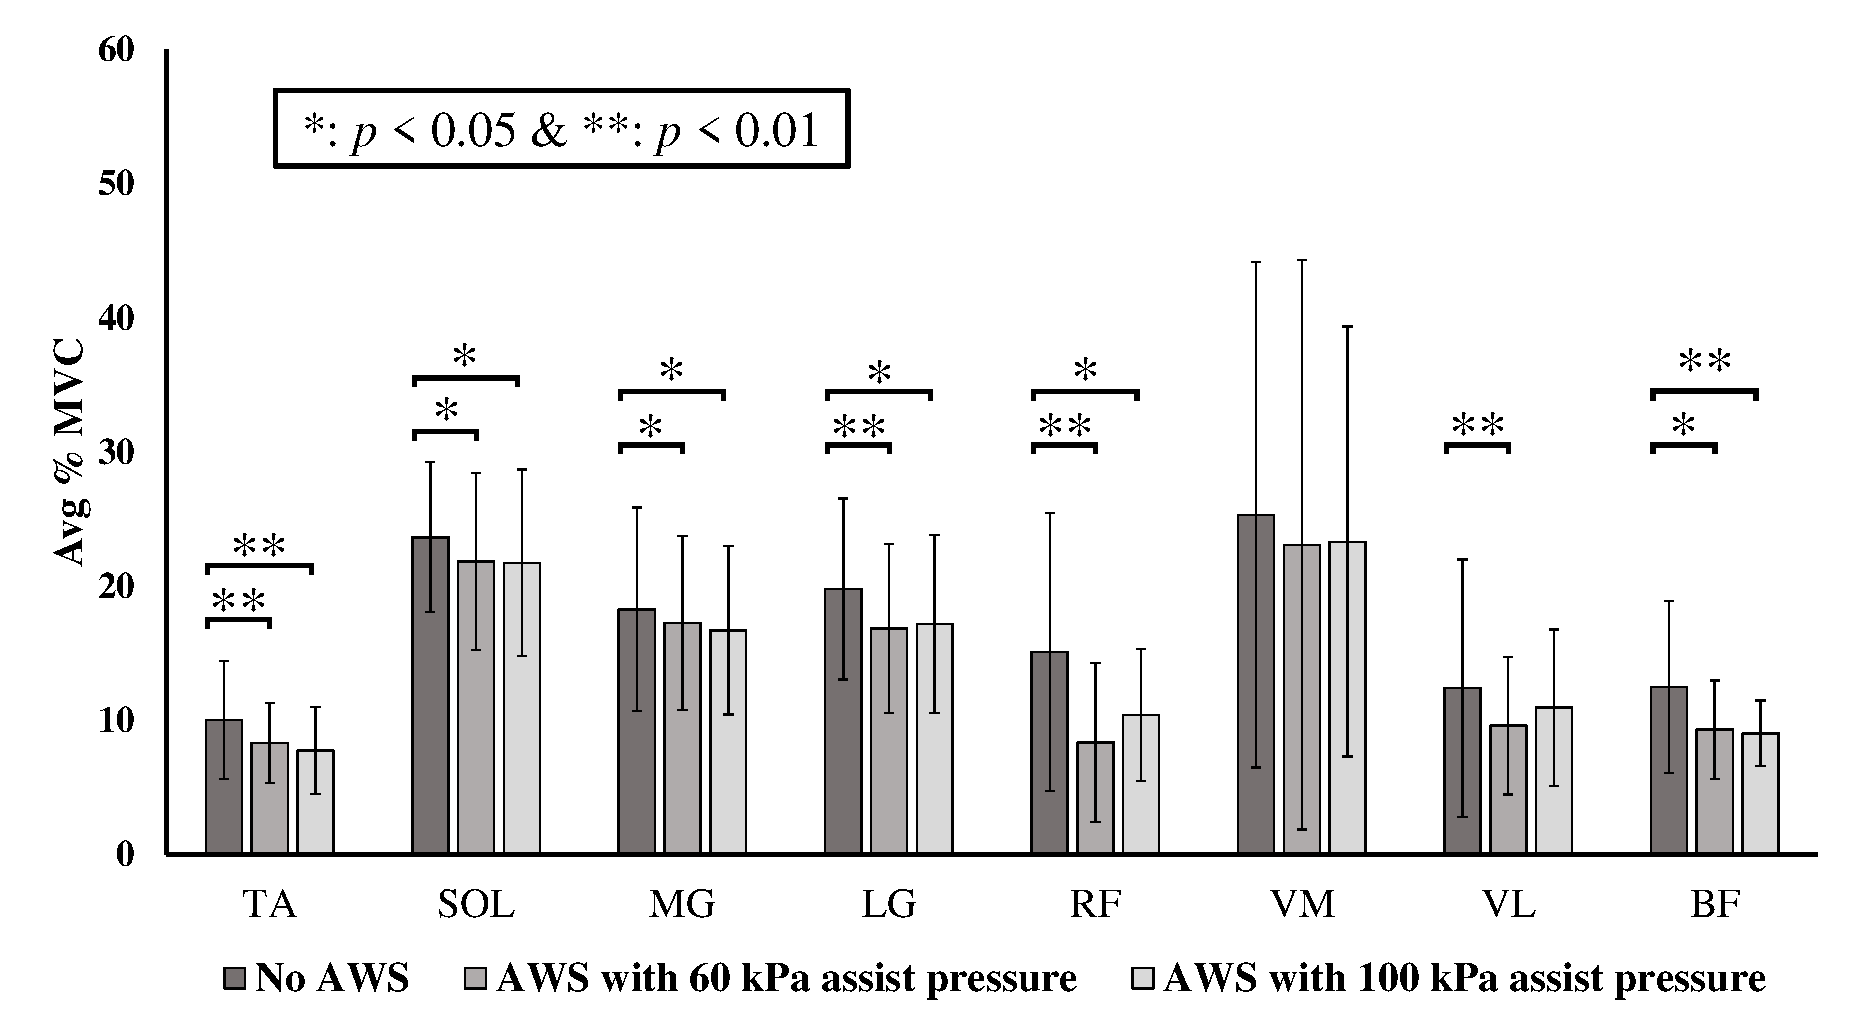
\includegraphics[width=0.9\linewidth]{../photos/aggregatedbargraph}
	\caption{The figure shows the significance of the reduction in \%MVC of the muscle groups for unassisted and assisted with two level of assistive force. The result shows significant reduction or no change in the muscle activation during assisted walking recorded for seven subjects.}
	\label{fig:aggregatedbargraph}
\end{figure*}

% Please add the following required packages to your document preamble:
% \usepackage{booktabs}
\begin{table}[]
	\centering
	\caption{Result of two sample t-test with the respective p-value, t-value and t-critical. p-value are maked with */** as displayed in Fig. \ref{fig:aggregatedbargraph}.}
	\label{t-test}
	\begin{tabular}{@{}cllcr@{}}
		\toprule
		\textbf{Muscles} & \multicolumn{1}{c}{\textbf{Experiment}} & \multicolumn{1}{c}{\textit{\textbf{p-value}}} & \textit{\textbf{t-value}} & \multicolumn{1}{c}{\textit{\textbf{t-critical}}} \\ \midrule
		TA               & AWS 60 Kpa                              & 0.0001 **                                     & 14.51                     & 2.78                                             \\
		& AWS 100 Kpa                             & 0.0002 **                                     & 24.25                     & 3.18                                             \\
		SOL              & AWS 60 Kpa                              & 0.0392 *                                      & 3.02                      & 2.78                                             \\
		& AWS 100 Kpa                             & 0.0329 *                                      & 3.20                      & 2.78                                             \\
		MG               & AWS 60 Kpa                              & 0.0310 *                                      & 3.85                      & 3.18                                             \\
		& AWS 100 Kpa                             & 0.0116 *                                      & 4.41                      & 2.78                                             \\
		LG               & AWS 60 Kpa                              & 0.0095 **                                     & 4.68                      & 2.78                                             \\
		& AWS 100 Kpa                             & 0.0201 *                                      & 4.53                      & 3.18                                             \\
		RF               & AWS 60 Kpa                              & 0.0079 **                                     & 6.35                      & 3.18                                             \\
		& AWS 100 Kpa                             & 0.0420 *                                      & 4.72                      & 4.30                                             \\
		VM               & AWS 60 Kpa                              & 0.0670                                        & 2.50                      & 2.78                                             \\
		& AWS 100 Kpa                             & 0.3300                                        & 1.16                      & 3.18                                             \\
		VL               & AWS 60 Kpa                              & 0.0075 **                                     & 6.46                      & 3.18                                             \\
		& AWS 100 Kpa                             & 0.4003                                        & 1.06                      & 4.30                                             \\
		BF               & AWS 60 Kpa                              & 0.0192 *                                      & 7.11                      & 4.30                                             \\
		& AWS 100 Kpa                             & 0.0020 **                                     & 10.16                     & 3.18                                             \\ \bottomrule
	\end{tabular}
\end{table}

\section{Discussion} \label{discuss}

Our results show that the previously developed PGM is used for the development of AWS and making it lightweight, portable and easy to use. The use of AWS showed a reduction in the muscle activity in all the major lower limb muscle. Due to the soft nature of the suit this device does not drastically disturb the normal gait of the wearer. 

The assistive control developed for AWS detect limbs going in the stance and swing phase during DLS by differentiating the FSR sensor data. This simple P control supports 20\%-30\% of the gait cycle during swing phase.  Due to the nature of the gait cycle and power source for the actuator, it is easy to add additional PGM’s to the AWS for increasing the range of assistive force. It is also possible to support stance and swing phase on a contralateral limb using same solenoid valve as in standard gait cycle both limbs functions synchronously.

The device uses waist and knee support to attach PGM along rectus femoris. This position sometimes causes little disturbance during walking. It can be addressed by changing the way PGM’s are attached to the limbs in a way such that it does not disturb degree of freedom (DOF) at the knee or any other joint PGM’s are used. 

The current state of the art wearable walking assist suits inspired by biological function of walking and the assistive actuators aligned with the muscles and joints of the lower limb \cite{8} .. \cite{13}. In such devices, the swing phase of the gait is assisted with actuators mechanism closed to the ankle or along soleus muscle and have demonstrated the reduction in the metabolic cost of walking. In our research, AWS is developed to assist swing phase by PGM  attached along RF muscle from hip to knee, and experimental evaluation shows a progressive reduction in the muscle activity of TA, SOL, MG, and LG. Along with this, RF VL and BF also show a reduction in muscle activity. However, changes in these muscle group show a decrease in change in muscle activity as we increase the assistive air pressure. These characteristics can be in Table \ref{percentred} and also from Fig. \ref{fig:aggregatedbargraph}. 

Qualitatively from the oral feedback from subjects, we found that the device is lightweight when not using 6 kg experimental setup; they also reported a feeling of the assistive force by PGM during the swing phase of the gait cycle. Some subject talked about feeling assistive force while walking when assistive air pressure changed to 100 kPa as compared to 60 kPa. They have reported that the PGM attachments do not disturb the walking experience much but improving the attachment at the knee can have a good feeling and better walking experience. 


% Please add the following required packages to your document preamble:
% \usepackage{booktabs}
\begin{table}[]
	\centering
	\caption{Reduction in \%MVC during assisted walking.}
	\label{percentred}
	\begin{tabular}{@{}ccc@{}}
		\toprule
		Muscle & \begin{tabular}[c]{@{}c@{}}60 kPa \\ Assistive Force\end{tabular} & \begin{tabular}[c]{@{}c@{}}100 kPa \\ Assitive Force\end{tabular} \\ \midrule
		TA     & 16.90\%                                                           & 22.70\%                                                           \\
		SOL    & 7.70\%                                                            & 8.10\%                                                            \\
		MG     & 5.50\%                                                            & 8.50\%                                                            \\
		LG     & 14.84\%                                                           & 13.10\%                                                           \\
		RF     & 44.00\%                                                           & 31\%                                                              \\
		VM     & 8.80\%                                                            & 7.90\%                                                            \\
		VL     & 22.50\%                                                           & 11.70\%                                                           \\
		BF     & 25.40\%                                                           & 27.60\%                                                           \\ \bottomrule
	\end{tabular}
\end{table}

\section{Conclusion and Future Work} \label{conclusion}

In this paper, we discussed the design, development, and evaluation of AWS to overcome the limitation of UPS regarding variable walking speed, easy to use and portability. To achieve this, we developed assistive control system by detecting limbs in the stance and swing phase during DLS phase of the gait cycle. The simple P control can switch on / off the assistive force during swing and stance phase respectively. While transitioning from UPS to AWS, the device weights 1.2 kg due to use of portable air tanks. We also demonstrated the ability to unload muscle efforts significantly by two levels of assistive force by AWS (comparing the sEMG for not wearing AWS and wearing AWS). 

Our evaluation show AWS unloads muscle efforts, during this process we found many areas for improvements and future tasks. In our result, we observe that for RF, VM, VL, and BF antagonistic behavior are seen. Increase in the assistive air pressure decreases reduction in muscle efforts; we would like to figure out the cause of such behavior in our further study and find the mechanism to cancel out such behavior. In our current study, we evaluate AWS using muscle activity changes, but the kinematic and physiological study is also essential for the evaluation of wearable assistive suit, we plan to conduct these studies in the future.  The assistive control of AWS uses FSR sensors in the shoe, the wires connecting for the shoe to the controller in the backpack causes little irritation to the user. We think the use of (inertial measurement unit) IMU sensors at the knee and ankle joint or flexible stretch sensors can provide information regarding gait cycle and similar assist control can be achieved. In the current implementation of the AWS, a backpack is used to keep the controller, battery, and air tank. In future, we want to integrate these in the waist support belt to make the device more user-friendly and easy to wear. 
We believe devices like these have enough opportunities for augmenting human walking for various age groups for augmented motion, rehabilitation and augmented sports and fun activities. To achieve it, further activities involves modeling of PGM assistive force characteristics and use it for dynamic assistive control and cancel out the negative effect on some of the muscle. 

\addtolength{\textheight}{-12cm}   % This command serves to balance the column lengths
% on the last page of the document manually. It shortens
% the textheight of the last page by a suitable amount.
% This command does not take effect until the next page
% so it should come on the page before the last. Make
% sure that you do not shorten the textheight too much.

%%%%%%%%%%%%%%%%%%%%%%%%%%%%%%%%%%%%%%%%%%%%%%%%%%%%%%%%%%%%%%%%%%%%%%%%%%%%%%%%



%%%%%%%%%%%%%%%%%%%%%%%%%%%%%%%%%%%%%%%%%%%%%%%%%%%%%%%%%%%%%%%%%%%%%%%%%%%%%%%%



%%%%%%%%%%%%%%%%%%%%%%%%%%%%%%%%%%%%%%%%%%%%%%%%%%%%%%%%%%%%%%%%%%%%%%%%%%%%%%%%

\section*{ACKNOWLEDGMENT}
The authors take this opportunity to thank members of Biological Systems Engineering lab at Graduate School of Engineering in Hiroshima University, Japan for participating in the performance evaluation of the AWS. We also like to thank Daiya Industries for supply and support for PGM development.  


\begin{thebibliography}{10}

\bibitem{1}	L. Garçon et al., “Medical and assistive health technology: Meeting the needs of aging populations,” Gerontologist, vol. 56, pp. S293–S302, 2016.
\bibitem{2}	K. Suzuki, G. Mito, H. Kawamoto, Y. Hasegawa, and Y. Sankai, “Intention-Based Walking Support for Paraplegia Patients with Robot Suit HAL,” Adv. Robot., vol. 21, no. 12, pp. 1441–1469, 2007.
\bibitem{3}	S. Toyama and G. Yamamoto, “Development of wearable-agri-robot - Mechanism for agricultural work,” in 2009 IEEE/RSJ International Conference on Intelligent Robots and Systems, IROS 2009, 2009, pp. 5801–5806.
\bibitem{4}	Y. Ikeuchi, J. Ashihara, Y. Hiki, H. Kudoh, and T. Noda, “Walking assist device with bodyweight support system,” in 2009 IEEE/RSJ International Conference on Intelligent Robots and Systems, IROS 2009, 2009, pp. 4073–4079.
\bibitem{5}	J. E. Pratt, B. T. Krupp, C. J. Morse, and S. H. Collins, “The RoboKnee: an exoskeleton for enhancing strength and endurance during walking,” in IEEE International Conference on Robotics and Automation, 2004. Proceedings. ICRA ’04. 2004, 2004, vol. 3, p. 2430–2435 Vol.3.
\bibitem{6}	P. Malcolm, W. Derave, S. Galle, and D. De Clercq, “A Simple Exoskeleton That Assists Plantarflexion Can Reduce the Metabolic Cost of Human Walking,” PLoS One, vol. 8, no. 2, 2013.
\bibitem{7}	B. T. Quinlivan et al., “Assistance magnitude versus metabolic cost reductions for a tethered multiarticular soft exosuit,” Sci. Robot., vol. 2, no. 2, p. eaah4416, 2017.
\bibitem{8}	A. T. Asbeck, K. Schmidt, and C. J. Walsh, “Soft exosuit for hip assistance,” Rob. Auton. Syst., vol. 73, pp. 102–110, 2015.
\bibitem{9}	K. Schmidt et al., “The myosuit: Bi-articular anti-gravity exosuit that reduces hip extensor activity in sitting transfers,” Front. Neurorobot., vol. 11, no. OCT, pp. 1–16, 2017.
\bibitem{10}	L. N. Awad et al., “A soft robotic exosuit improves walking in patients after stroke,” Sci. Transl. Med., vol. 9, no. 400, 2017.
\bibitem{11}	S. Sridar, P. H. Nguyen, M. Zhu, Q. P. Lam, and P. Polygerinos, “Development of a soft-inflatable exosuit for knee rehabilitation,” IEEE Int. Conf. Intell. Robot. Syst., vol. 2017–Septe, pp. 3722–3727, 2017.
\bibitem{12}	A. T. Asbeck, S. M. M. De Rossi, K. G. Holt, and C. J. Walsh, “A biologically inspired soft exosuit for walking assistance,” Int. J. Rob. Res., vol. 34, no. 6, pp. 744–762, 2015.
\bibitem{13}	S. H. Collins, M. B. Wiggin, and G. S. Sawicki, “Reducing the energy cost of human walking using an unpowered exoskeleton,” Nature, vol. 522, no. 7555, pp. 212–215, 2015.
\bibitem{14}	K. Ogawa, C. Thakur, T. Ikeda, T. Tsuji, and Y. Kurita, “Development of a pneumatic artificial muscle driven by low pressure and its application to the unplugged powered suit,” Adv. Robot., vol. 31, no. 21, pp. 1135–1143, 2017.
\bibitem{15}	F. Daerden and D. Lefeber, “Pneumatic artificial muscles: actuators for robotics and automation,” Eur. J. Mech. Environ. Eng., vol. 47, no. 1, pp. 11–21, 2002.
\bibitem{16}	C. Thakur, K. Ogawa, T. Tsuj, and Y. Kurita, “Unplugged powered suit with pneumatic gel muscles,” in Lecture Notes in Electrical Engineering, 2018, vol. 432, pp. 247–251.
\bibitem{17}	R. W. Kressig and O. Beauchet, “Guidelines for clinical applications of spatio-temporal gait analysis in older adults,” Aging Clin. Exp. Res., vol. 18, no. 2, pp. 174–176, Apr. 2006.


\end{thebibliography}
\end{document}
